\documentclass{article}

\usepackage[utf8]{inputenc}
\usepackage{tikz}
\usepackage{pgfplots}
\pgfplotsset{compat=1.10}
\usetikzlibrary{calc, patterns}
\usepgfplotslibrary{fillbetween}

\title{Plottting Ticz}
\author{JV}
\begin{document}
\maketitle


This is a test paragraph.

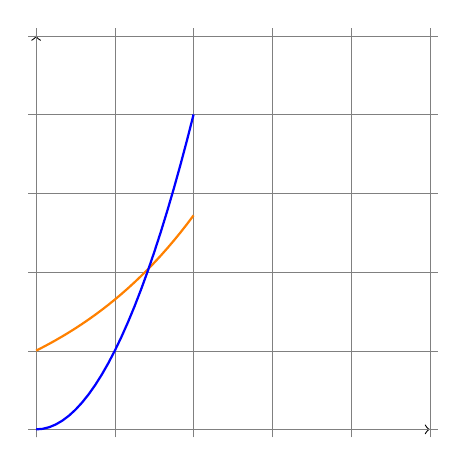
\begin{tikzpicture}
    \draw[->] (-0.1, 0) -- (5.0,0);
    \draw[->] (0, -0.1) -- (0,5.0); 
    \draw[gray, ultra thin] (-0.1, -0.1) grid (5.1,5.1); 
    \draw[domain=0:2, orange, thick] plot (\x, {exp(\x/2)});
    \draw[domain=0:2, blue, thick] plot (\x, {\x*\x});
\end{tikzpicture}

We define domain on top near tikzpicture below:

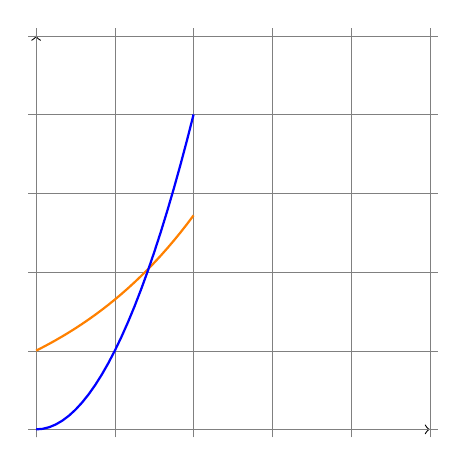
\begin{tikzpicture}[domain = 0:2]
    \draw[->] (-0.1, 0) -- (5.0,0);
    \draw[->] (0, -0.1) -- (0,5.0); 
    \draw[gray, ultra thin] (-0.1, -0.1) grid (5.1,5.1); 
    \draw[ orange, thick] plot (\x, {exp(\x/2)});
    \draw[ blue, thick] plot (\x, {\x*\x});
\end{tikzpicture}

\pagebreak

Label like this below:

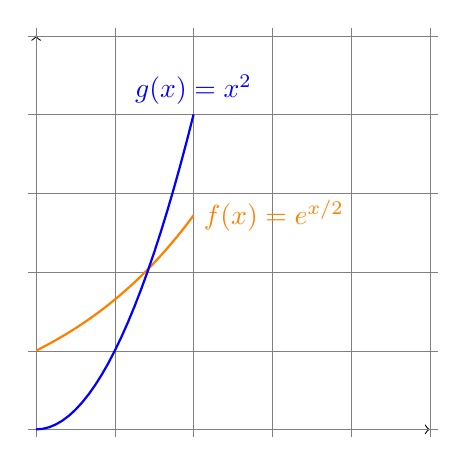
\begin{tikzpicture}[domain = 0:2]
    \draw[->] (-0.1, 0) -- (5.0,0);
    \draw[->] (0, -0.1) -- (0,5.0); 
    \draw[gray, ultra thin] (-0.1, -0.1) grid (5.1,5.1);
    \draw[ orange, thick] plot (\x, {exp(\x/2)}) node[right]{$f(x) = e^{x/2}$};
    \draw[ blue, thick] plot (\x, {\x*\x}) node[above] {$g(x) = {x^2}$};
\end{tikzpicture}

Center this picture:

\begin{center}
    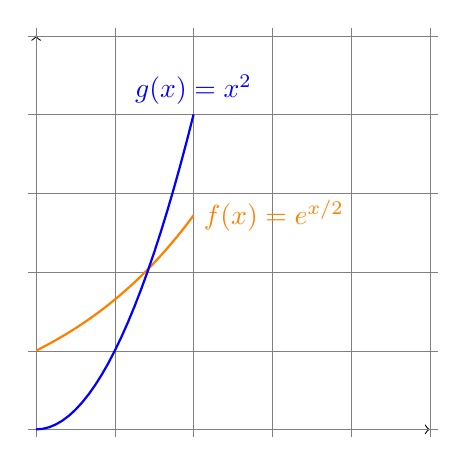
\begin{tikzpicture}[domain = 0:2]
        \draw[->] (-0.1, 0) -- (5.0,0);
        \draw[->] (0, -0.1) -- (0,5.0); 
        \draw[gray, ultra thin] (-0.1, -0.1) grid (5.1,5.1);
        \draw[ orange, thick] plot (\x, {exp(\x/2)}) node[right]{$f(x) = e^{x/2}$};
        \draw[ blue, thick] plot (\x, {\x*\x}) node[above] {$g(x) = {x^2}$};
    \end{tikzpicture}    
\end{center}

See the coordinate system:

\begin{center}
    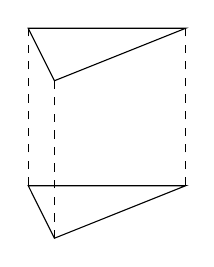
\begin{tikzpicture}[domain = 0:2]
        \coordinate (A) at (-1, 0, 0);
        \coordinate (B) at ( 1, 0, 0);
        \coordinate (C) at (0, 0, {sqrt(3)});
        \coordinate (H) at (0, 2, 0);
        \draw (B) -- (C) -- (A) -- cycle;
        \draw ($(B)+(H)$) -- ($(C)+(H)$) -- ($(A)+(H)$) -- cycle;
        \draw[dashed] (A)  -- ($(A) + (H)$);
        \draw[dashed] (B)  -- ($(B) + (H)$);
        \draw[dashed] (C)  -- ($(C) + (H)$);
    \end{tikzpicture}
    \end{center}

\pagebreak
Integral thing (dashed area):

\begin{center}
    \begin{tikzpicture}[domain = 0:2]
        \draw[->, thick] (-1, 0) -- (3.0, 0);
        \draw[->, thick] (0, -1) -- (0, 3.0); 
        %\draw[gray, ultra thin] (-1, -1) grid (3,5);
        \draw[ blue, thick] plot (\x, {exp(\x/2)}) node[right]{$f(x) = e^{x/2}$};
        \draw[dashed] (1, 0) -- (1,  {exp(1/2)});
        \draw[dashed] (2, 0) -- (2,  {exp(2/2)});

    \end{tikzpicture}    
\end{center}

Integral with shaded area:


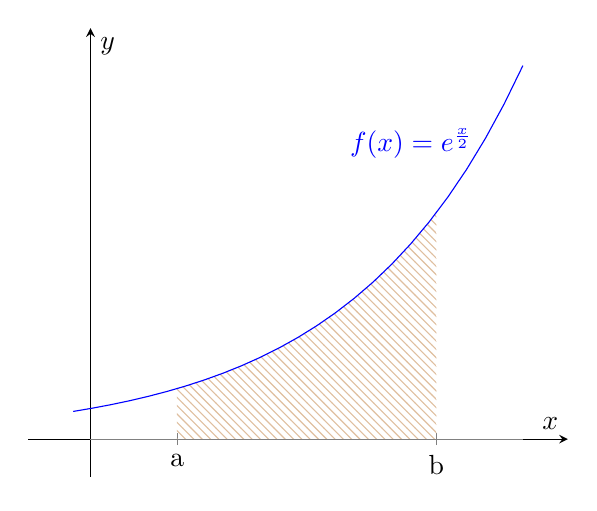
\begin{tikzpicture}[domain = 0:2]
    \begin{axis}[axis lines=middle,
        xlabel=$x$,
        ylabel=$y$,
        enlargelimits,
        ytick=\empty,
        xtick={1,4},
        xticklabels={a,b}]
    \addplot[name path=F,blue,domain={-.2:5}] {exp(\x/2)} node[pos=0.8, left]{$f(x) = e^{\frac{x}{2}}$};
    \addplot[name path=G,gray, thin,domain={0:5}] {0};
    \addplot[pattern=north west lines, pattern color=brown!50]fill between[of=F and G, soft clip={domain=1:4}];
    \end{axis}
\end{tikzpicture}    

\pagebreak

Integral with shaded area, with figure:

\begin{figure}[h]
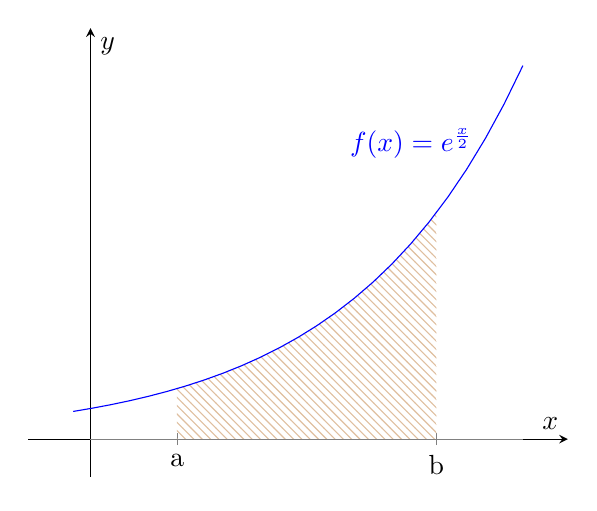
\begin{tikzpicture}[domain = 0:2]
    \begin{axis}[axis lines=middle,
        xlabel=$x$,
        ylabel=$y$,
        enlargelimits,
        ytick=\empty,
        xtick={1,4},
        xticklabels={a,b}]
    \addplot[name path=F,blue,domain={-.2:5}] {exp(\x/2)} node[pos=0.8, left]{$f(x) = e^{\frac{x}{2}}$};
    \addplot[name path=G,gray, thin,domain={0:5}] {0};
    \addplot[pattern=north west lines, pattern color=brown!50]fill between[of=F and G, soft clip={domain=1:4}];
    \end{axis}
\end{tikzpicture}
\caption{This is Area under the curve}
\end{figure}

Integral with shaded area, with figure and centering:

\begin{figure}[h]
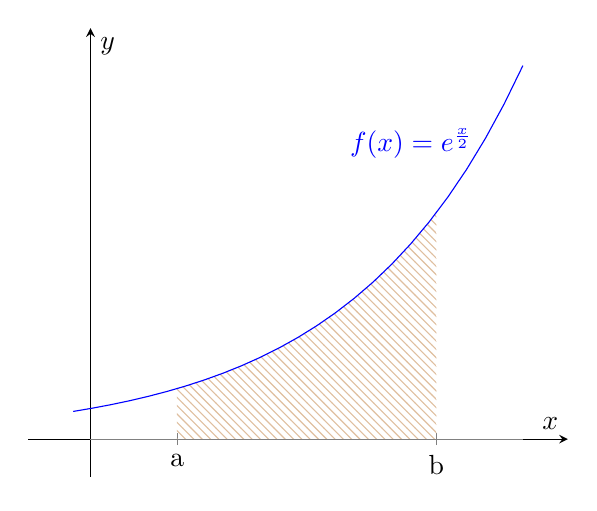
\begin{tikzpicture}[domain = 0:2]
    \begin{axis}[axis lines=middle,
        xlabel=$x$,
        ylabel=$y$,
        enlargelimits,
        ytick=\empty,
        xtick={1,4},
        xticklabels={a,b}]
    \addplot[name path=F,blue,domain={-.2:5}] {exp(\x/2)} node[pos=0.8, left]{$f(x) = e^{\frac{x}{2}}$};
    \addplot[name path=G,gray, thin,domain={0:5}] {0};
    \addplot[pattern=north west lines, pattern color=brown!50]fill between[of=F and G, soft clip={domain=1:4}];
    \end{axis}
\end{tikzpicture}
\caption{This is Area under the curve}
\end{figure}

\pagebreak
With polynomial kind :

\begin{figure}[h]
    \begin{tikzpicture}[domain = -5:5]
        \begin{axis}[axis lines=middle,
            xlabel=$x$,
            ylabel=$y $,
            enlargelimits,
            ytick=\empty,
            xtick={-3,1,4},
            xticklabels={-3,1,2}]
        \addplot[name path=F,blue,domain={-3.5:5}] {(\x+3)*(\x-1)*(\x-4)} node[pos=0.8, left]{$f(x) = (x+3)(x-1)(x-2)$};
        \end{axis}
    \end{tikzpicture}
    \caption{Cubic Polynomial}
    \end{figure}


\end{document}